\chapter{Introduction}\label{chap:intro}

\section{Background}

With the recent advances in data-as-a-service (DaaS) and cloud computing, outsourcing data to the cloud has become the common practice. In a typical scenario shown in \Cref{fig:intro:model}, the \emph{data owner} (DO) outsources the data to a third party in the cloud known as \emph{service provider} (SP). Upon receiving the query requests from the clients, the SP will process them on the behavior of the DO\@. Since the SP has more computation power and storage capability than those of the DO, such cloud outsourcing paradigm is able to scale up the services with a low cost. However, as the SP is often a third-party delegate of the DO, it cannot be trusted. For example, the SP may return tampered or partial results due to a variety of reasons including service outages, hack attacks, or even corporate dishonesty. Therefore, it is important to authenticate the query results such that the clients can verify their soundness (all results are genuine) and completeness (no result is missing).

\begin{figure}[h]
  \centering
  \resizebox{.7\linewidth}{!}{\begin{tikzpicture}
  \node [scale=1] (do) {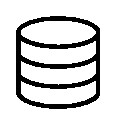
\includegraphics{./figs/icons/database.eps}};
  \node [scale=1,right=2cm of do](sp){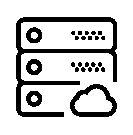
\includegraphics{./figs/icons/server.eps}};
  \node [scale=2,right=2cm of sp](client){
\includegraphics{./figs/icons/user.eps}};
  \draw[-latex] (do.east) -- (sp.west) node [midway,above,font=\scriptsize] {Data \& ADS};
  \draw[-latex,transform canvas={yshift=0.5ex}] (client.west) -- (sp.east) node [midway,above,font=\scriptsize] {Queries};
  \draw[-latex,transform canvas={yshift=-0.5ex}] (sp.east) -- (client.west) node [midway,below,font=\scriptsize] {Results \& VO};
  \node [font=\footnotesize,below=0cm of sp](sp-label){\textbf{Services Provider (SP)}};
  \node [font=\footnotesize] at (do |- sp-label) {\textbf{Data Owner (DO)}};
  \node [font=\footnotesize] at (client |- sp-label) {\textbf{Clients}};
\end{tikzpicture}
}
  \caption{Authenticated Query Processing System Model}\label{fig:intro:model}
\end{figure}

In the field of query processing, query authentication has been studied by a large body of literature~\cite{10.1109/ICDE.2004.1320027,10.1145/1142473.1142488,10.1007/s00778-008-0113-2,10.1145/1880022.1880026,10.1145/2213836.2213871,10.1145/2463676.2465281,10.14778/2732219.2732224,10.1145/2664243.2664244,10.1145/2723372.2747649,10.1109/tkde.2014.2316818}. The fundamental concept is that the DO signs a well-designed \emph{authenticated data structure} (ADS) as notarization of the outsourced data. Based on the ADS, the SP then constructs a cryptographic proof, known as \emph{verification object} (VO), for each query, and returns it along with the query results for the client to verify.

However, the prior works only consider to support primitive queries.

To address these issues, in this dissertation, we take the first step to study three new problems, namely
\begin{inlineenum}
  \item authentication of aggregate queries over set-valued data,
  \item authentication of relational queries with fine-grained access control, and
  \item authentication of {kNN} queries in distributed environment.
\end{inlineenum}

\section{Authenticating Aggregate Queries over Set-Valued Data}

\section{Authenticating Relational Queries with Fine-Grained Access Control}

\section{Authenticating {kNN} Queries in Distributed Environment}

\section{Dissertation Outline}

The rest of the dissertation is organized as follows. \Cref{chap:related-works} reviews existing studies. \Cref{chap:aggregate-queries} presents the authentication of aggregate queries over set-valued data. \Cref{chap:access-control} studies the authentication of relation queries with fine-grained access control. The authentication of kNN queries in distributed environment is investigated in \Cref{chap:knn}. Finally, the dissertation is concluded in \Cref{chap:conclusions}.
